\section{Design}

\subsection{Barrel layout and support structure}

SVT comprises 21504 channels of silicon strip sensors in six layers (three concentric polygonal regions that have 10, 14, and 18 double sided modules). The SVT is enclosed by the Faraday cage with inner radius of 57 mm (with 6 mm clearance to the target scattering chamber) and the outer radius of 133 mm. To minimize multiple scattering a unique module design with extra long 33~cm strips has been developed to reduce material budget to about 1.4$\%$ of radiation length per region (two silicon planes) for normal incidence tracks, which is essential for tracking at low momenta~\cite{Vertex2016}. 

\begin{figure}[hbt] 
\centering 
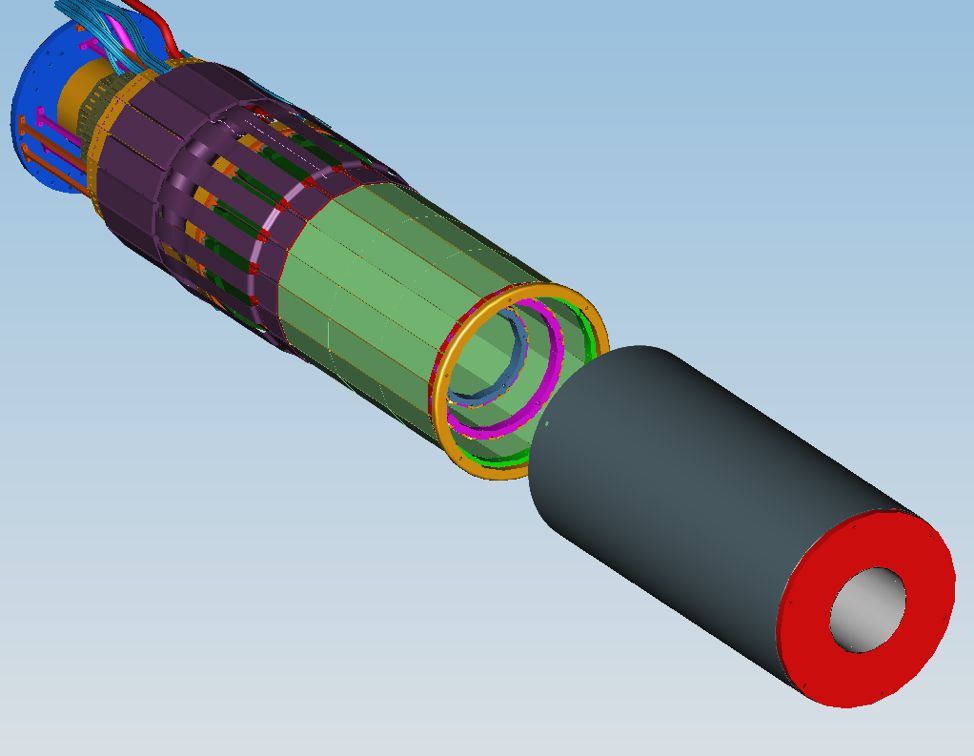
\includegraphics[width=1.0\columnwidth,keepaspectratio]{barrel-faradaycage.png}
\caption{Layout of the barrel and the Faraday Cage. Copper supports shown in yellow.  Supports are bolted directly to cold plate. Silicon sensors are shown in green.}
\label{fig:barrel-faradaycage}
\end{figure}

All SVT modules are made identical to minimize the production cost. There are no overlaps of adjacent modules.

%\begin{wrapfigure}{l}{0.5\columnwidth}
%\centering 
%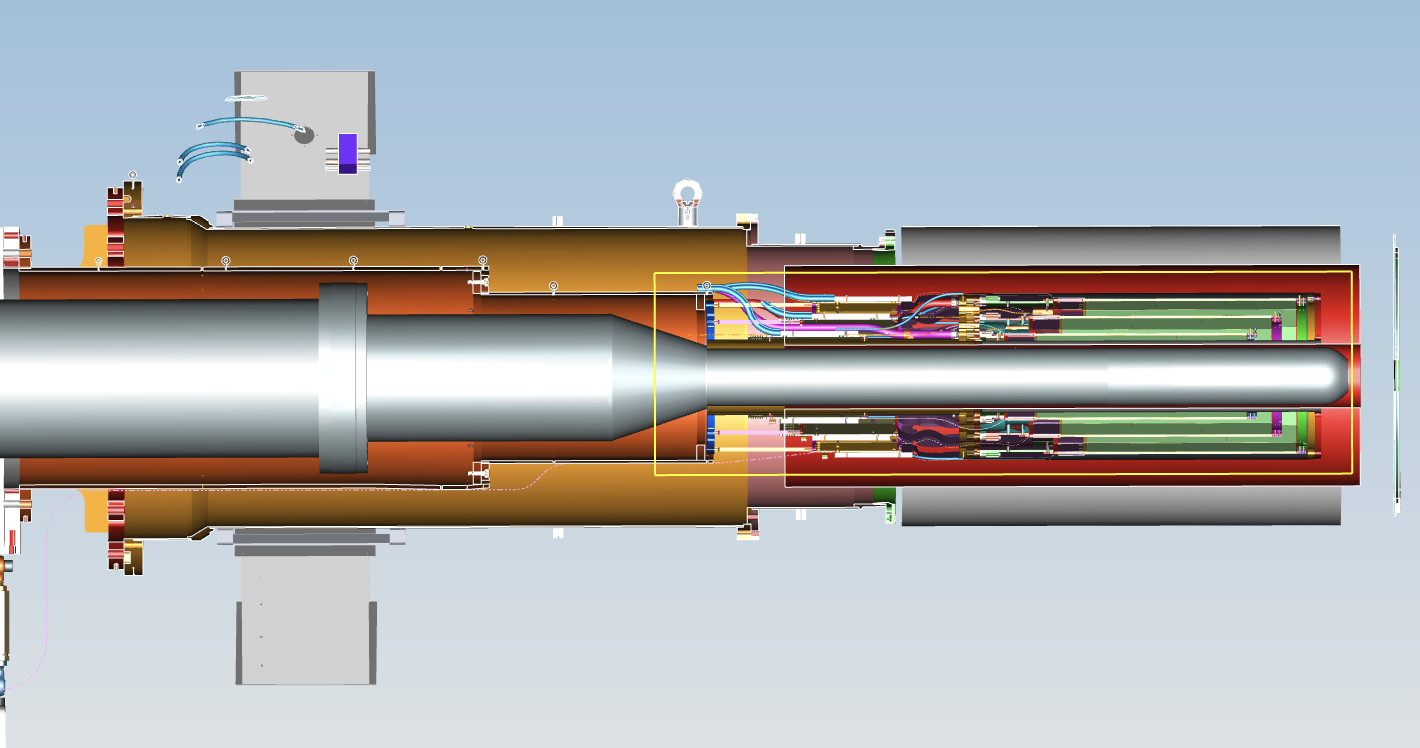
\includegraphics[width=1.0\columnwidth]{cvt-crosssection.png}
%\caption{CVT crossection.}
%\label{fig:cvt-crosssection}
%\end{wrapfigure}

%Figure~\ref{fig:cvt-crosssection} shows the side view of the detector. 

The modules  are mounted between the upstream and the downstream rings (Fig.~\ref{fig:barrel-faradaycage}). For each region the upstream ring is attached to the cold plate with screws. The upstream support ring provides a mounting surface for the modules on the upstream end of the detector. It also provides a conduction path for heat to be transferred from the modules to the coolant flowing through the cold plate. 

\begin{figure}[hbt] 
\centering 
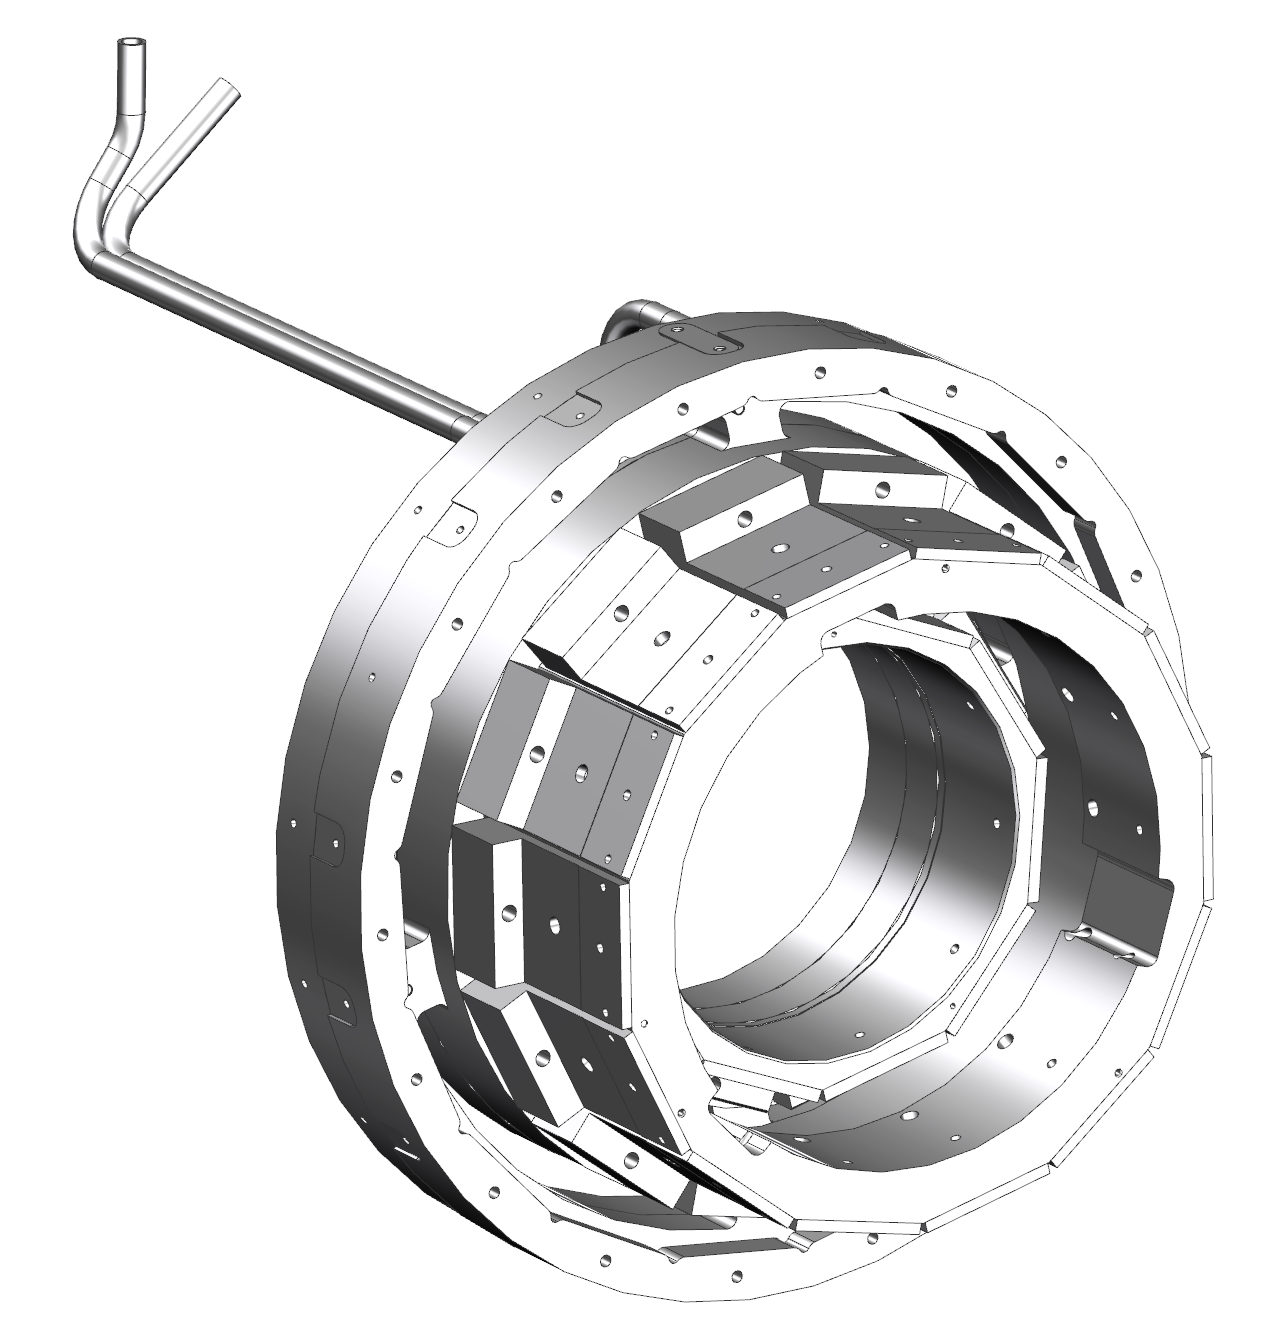
\includegraphics[width=1.0\columnwidth,keepaspectratio]{upstreamring.png}
\caption{Upstream support ring attached to the cold plate.}
\label{fig:upstreamring}
\end{figure}

 The SVT modules are cantilevered off a chilled cold plate, designed to provide mechanical support and remove heat generated by the electronics, located at the upstream end of the module outside of the tracking volume (Figure~\ref{fig:upstreamring}). The cold plate is bolted to the mounting tube which is attached to the insertion cart with the support tube. 
 
The cold plate and upstream ring are attached to the mounting tube. The mounting surfaces of the upstream and downstream rings are machined closely coupled in a single step to guarantee planarity. The rings of each region are independent from each other to prevent over-constraining the assembly. This design allows an entire region to be removed as a unit, rather than module by module. The modules in the vertical and near vertical position provide stiffness to the downstream ring and to a region as a whole. Regions are shifted along the beam axis to ensure angular coverage. Downstream rings are made of PolyEther Ether Ketone (PEEK)~\cite{NIMVCC}. 

\begin{figure}[hbt] 
\centering 
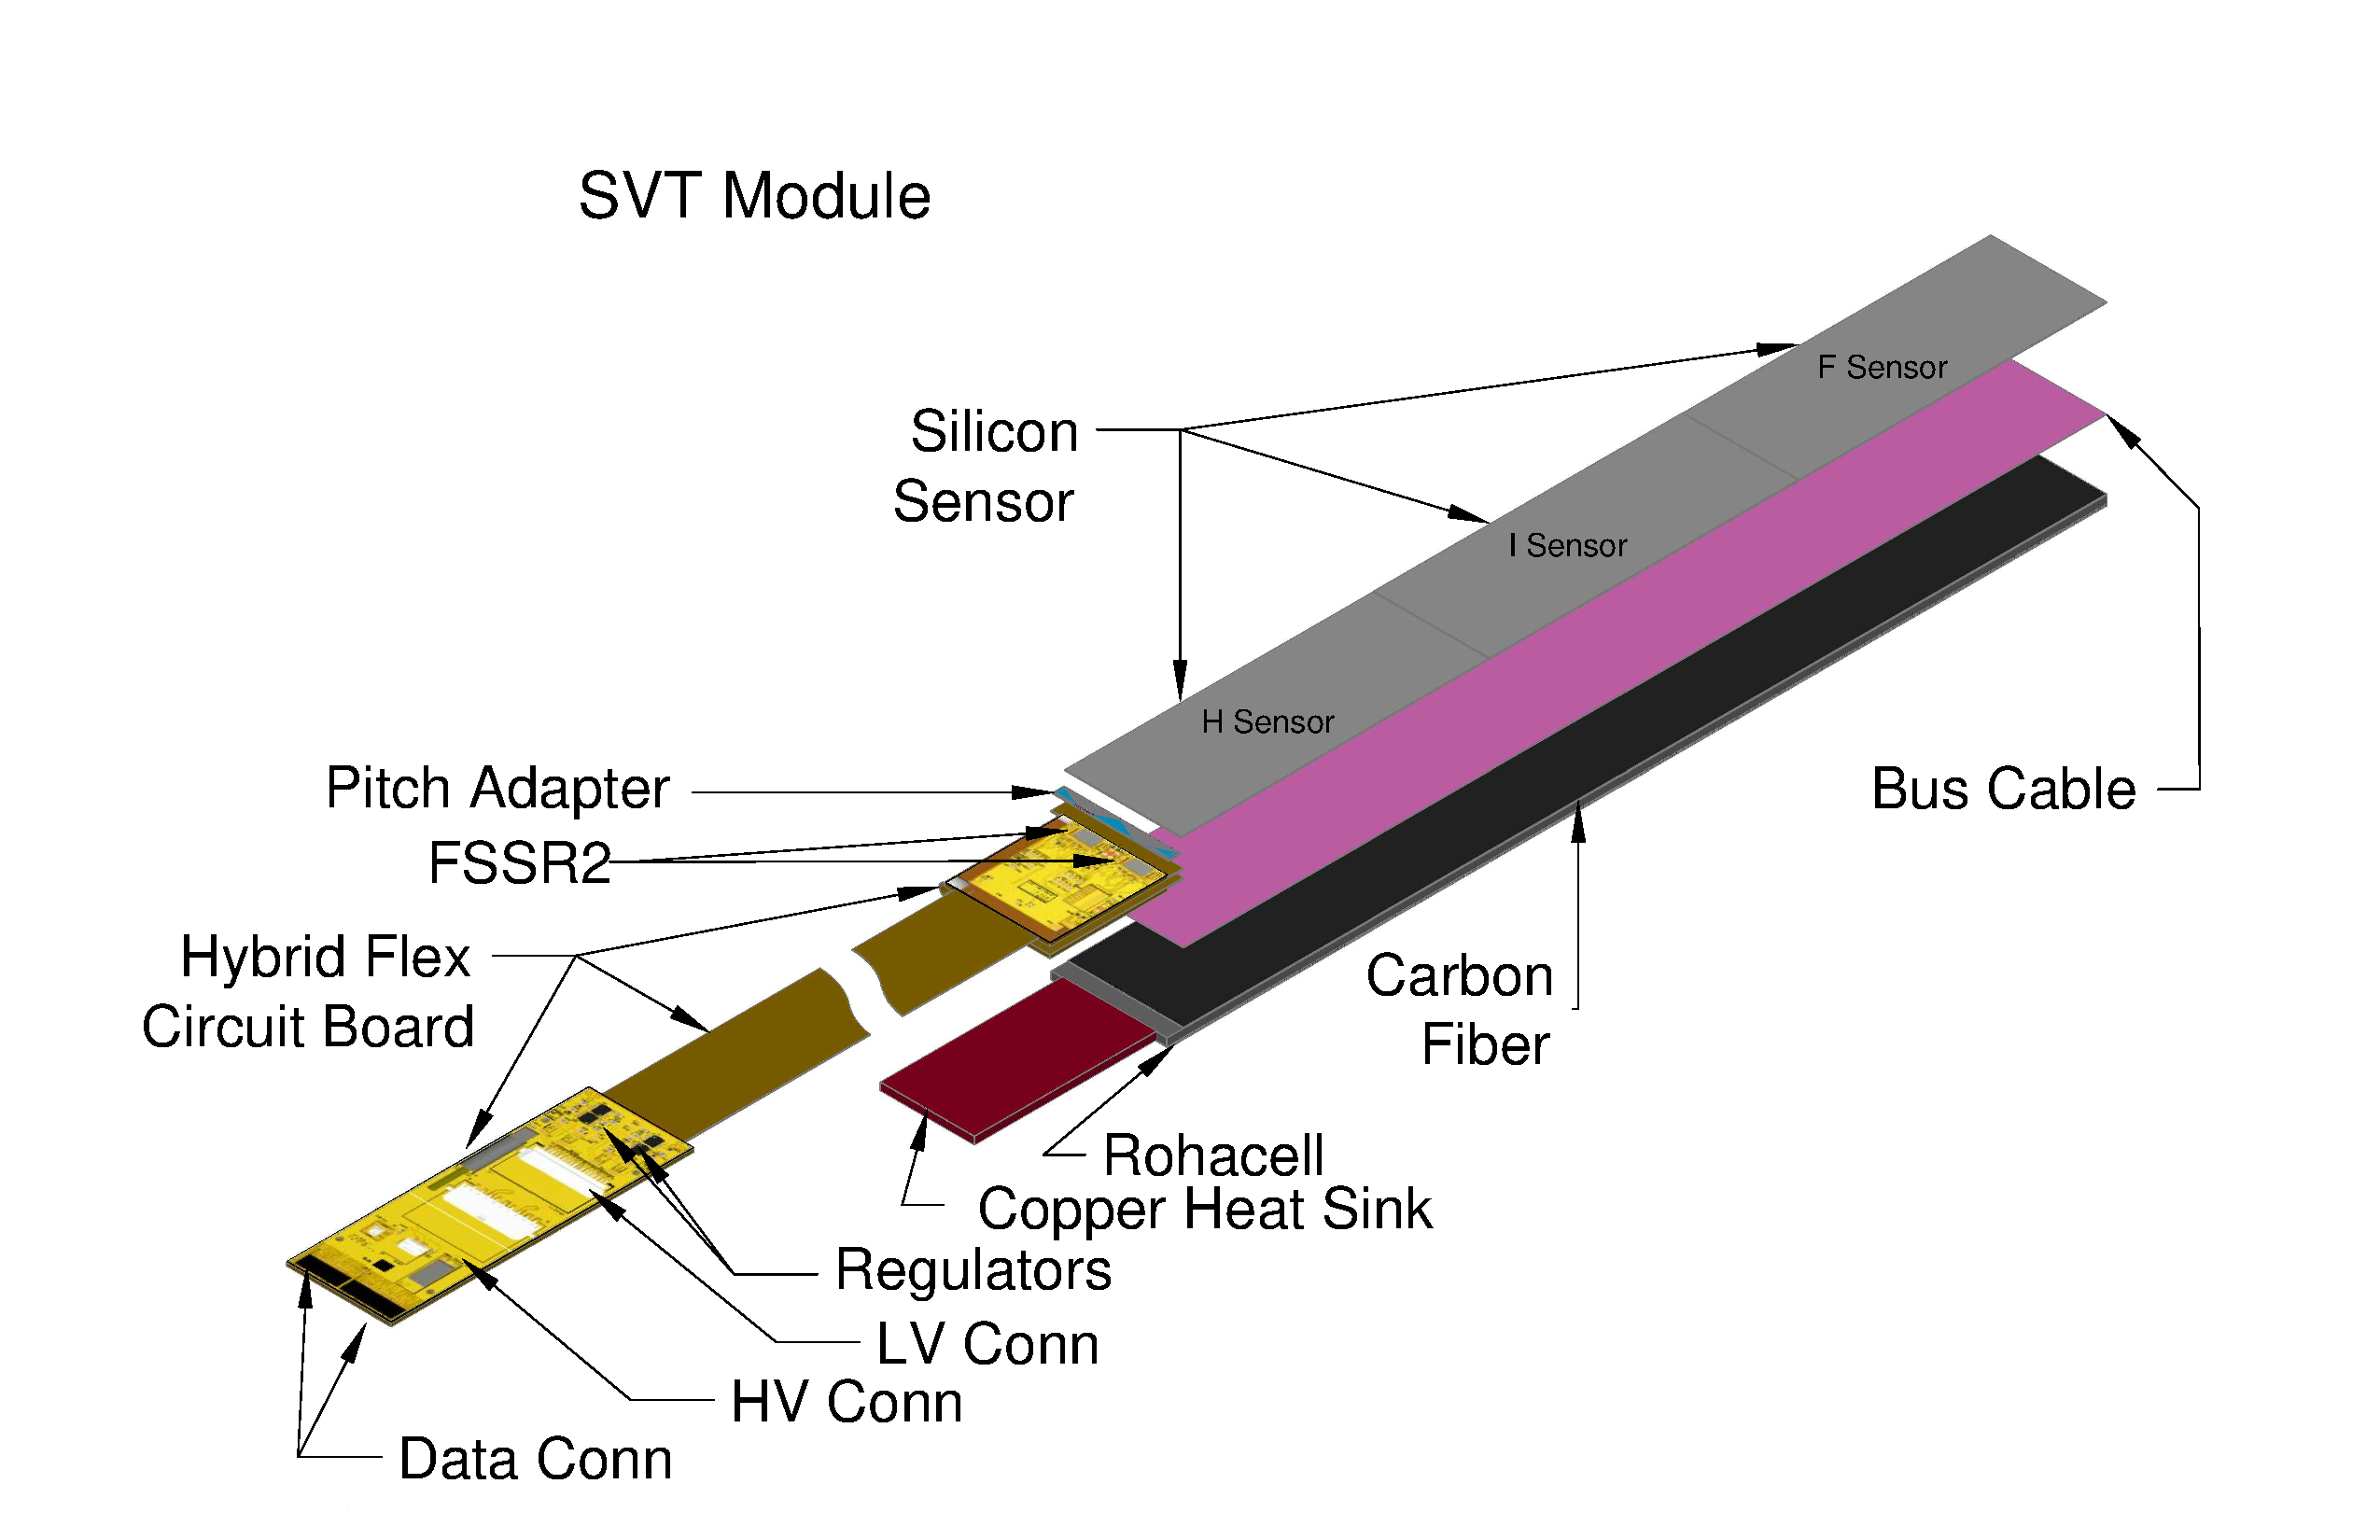
\includegraphics[width=1.0\columnwidth,keepaspectratio]{module.pdf}
\caption{Layout of the SVT module.}
\label{fig:module}
\end{figure}

\subsection{Module design}

SVT uses single sided 320~$\mu$m thick microstrip sensors fabricated by Hamamatsu mounted on each side of the module (see Fig.~\ref{fig:module}). All modules have 3 types of sensors: H (Hybrid), I (Intermediate), and F (Far). Sensors are cut from 6 inch wafers, 2 sensors per wafer to maximize the yield. All sensors have the same size, 112$\times$42 mm. There are three daisy-chained sensors per layer (six per module) with 110~$\mu$m gap between them. 

\begin{figure}[hbt] 
\centering 
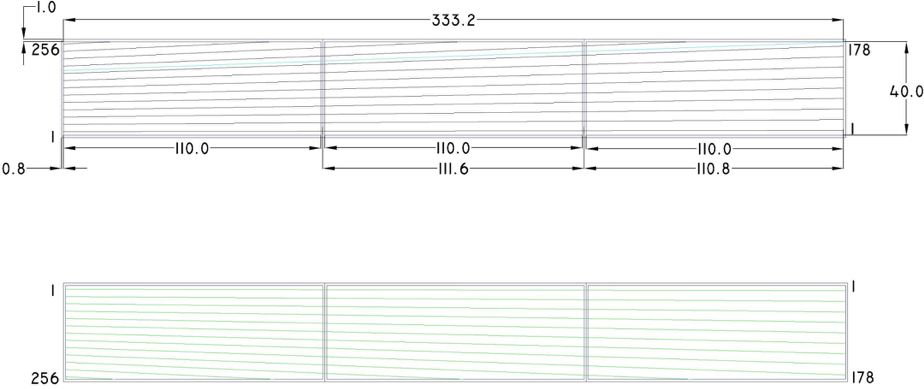
\includegraphics[width=1.0\columnwidth,keepaspectratio]{strip-layout.png}
\caption{Sensor strip layout.}
\label{fig:strip-layout}
\end{figure}

Each layer has 256 strips with linearly varying angles of 0$^\circ$--3$^\circ$ (constant $\phi$ pitch of 1/85$^\circ$) to minimize dead sensor area. First readout strip is parallel to the longitudinal axis of the module; the last readout strip has an angle of 3$^\circ$ with respect to this axis (see Fig.~\ref{fig:strip-layout}). Because of the constant $\phi$ pitch, the lengths of the readout strips of the modules vary from 0.5 cm to 33 cm. At the hybrid side the intermediate strip pitch is 78 $\mu$m and the readout pitch is 156 $\mu$m The strip-to-pitch ratio is 0.256 for all three types of sensors.

\begin{figure}[hbt] 
\centering 
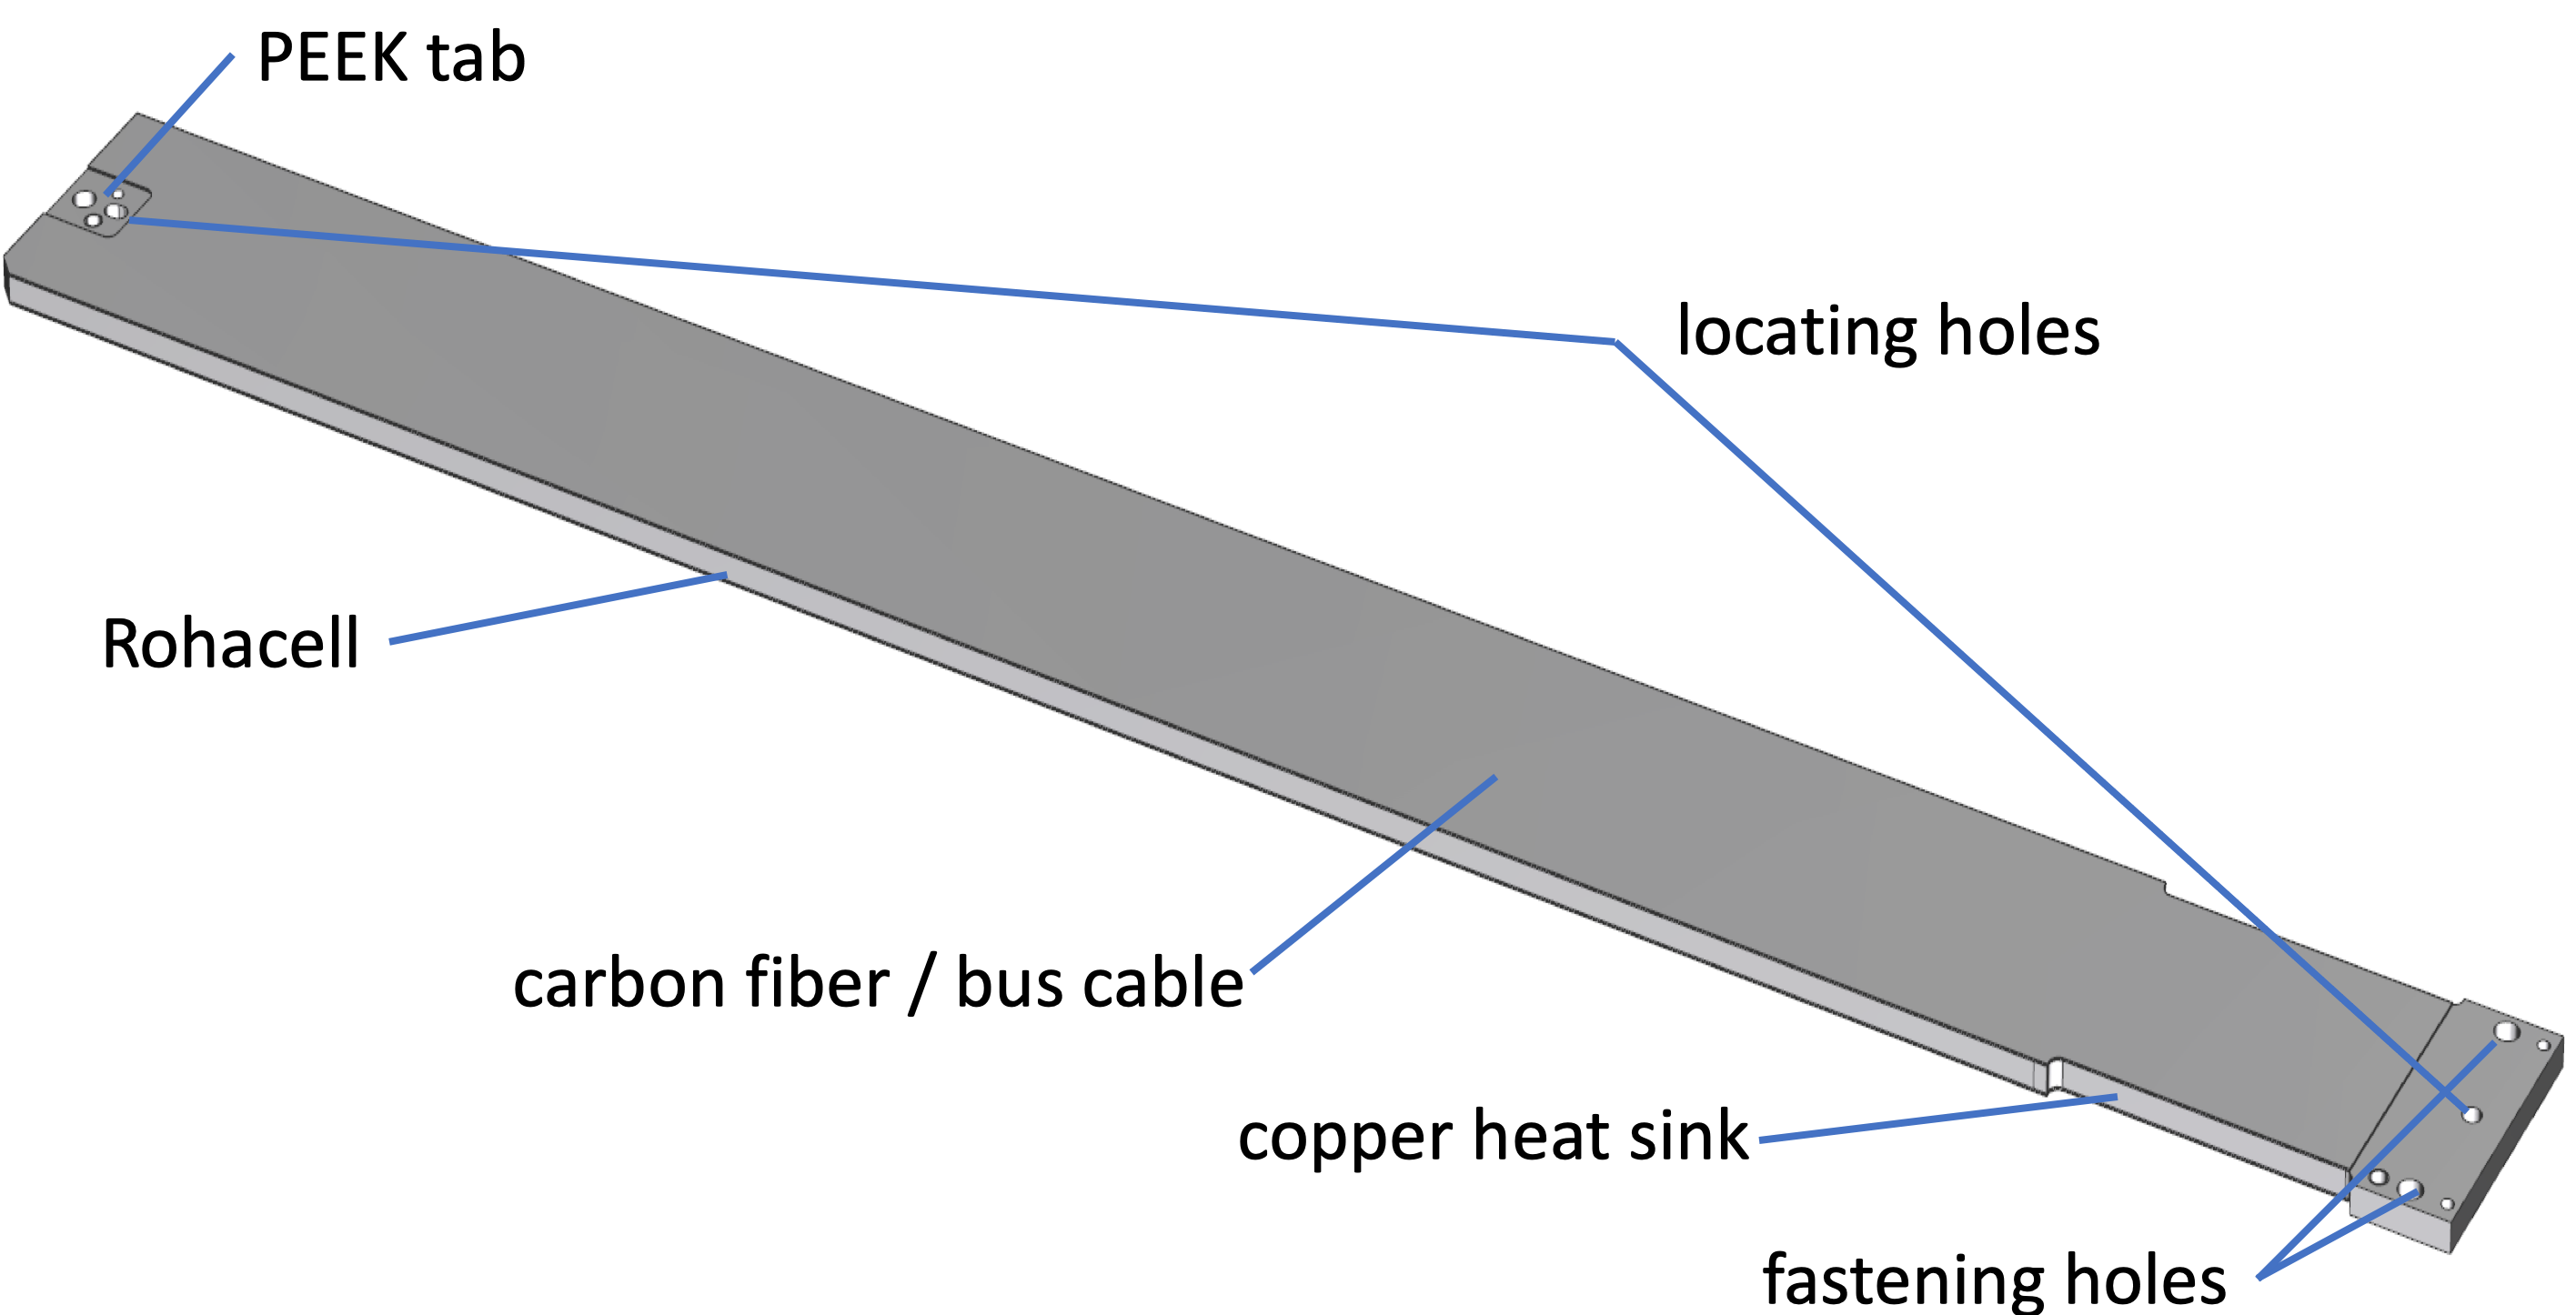
\includegraphics[width=1.0\columnwidth,keepaspectratio]{backing-structure.png}
\caption{Backing structure.}
\label{fig:backing-structure}
\end{figure}

Sensors are mounted on a backing structure composed of Rohacell 71 core, bus cable, and carbon fiber (see Fig.~\ref{fig:backing-structure}). The carbon fiber skin is made from Mitsubishi type K13C2U fibers oriented in a quasi-isotropic (45/-45/0) pattern. To ensure adequate electrical conductivity it is co-cured with the bus cable, made from a Kapton sheet with 3 $\mu$m thick and 0.5~mm wide copper traces; one side provides high voltage to the sensors, a 6$\times$6~mm copper mesh on another side grounds the carbon fiber.  The Rohacell core under the hybrid board is replaced by a copper heat sink to remove $\sim$2~W of heat generated by the ASICs. At the downstream end of the module, the Rohacell core is replaced by a PEEK insert.  

\begin{figure}[hbt] 
\centering 
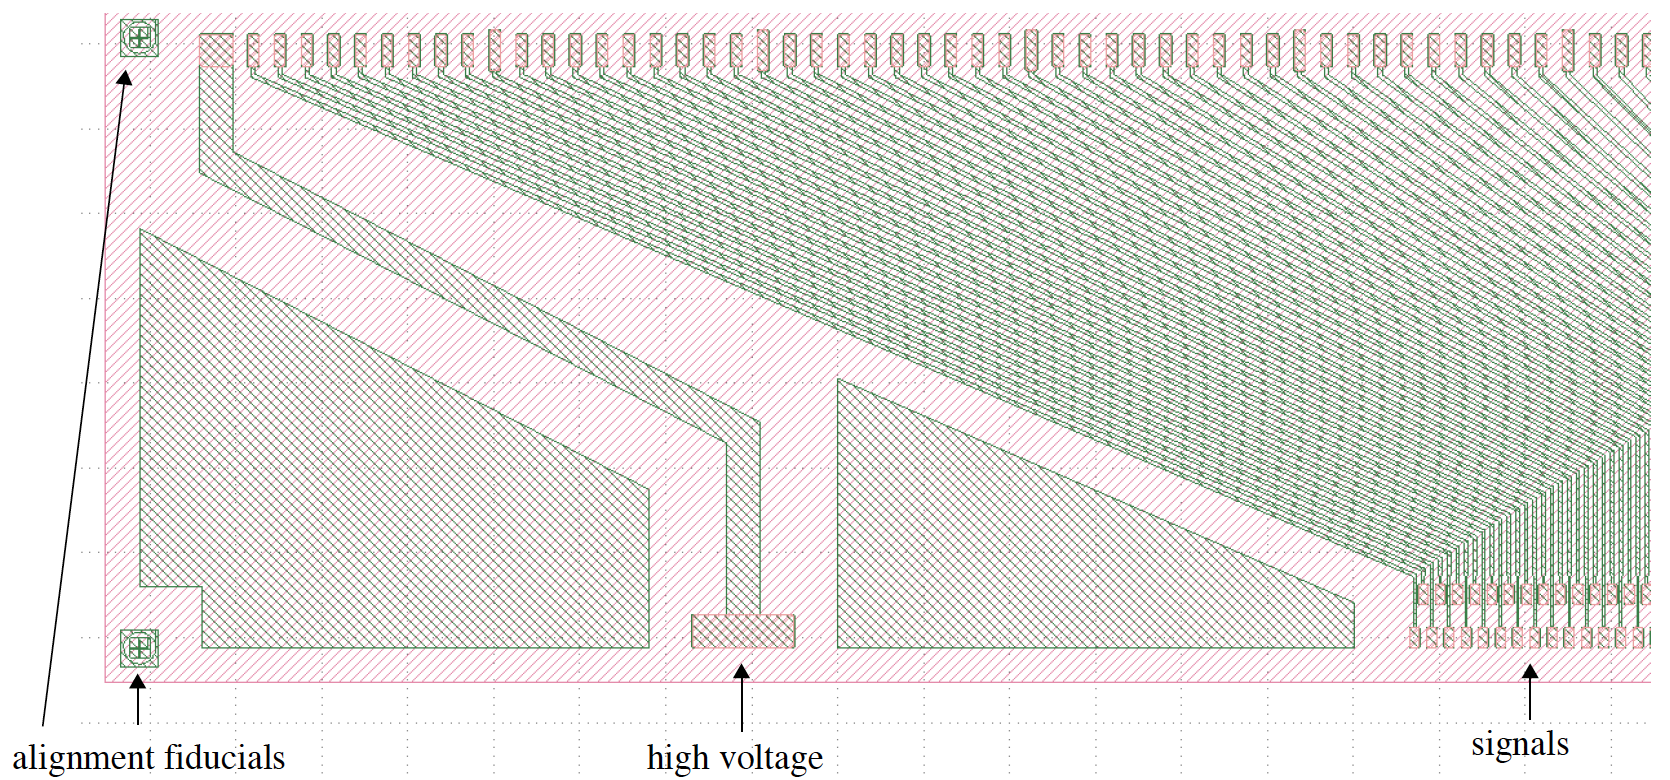
\includegraphics[width=1.0\columnwidth,keepaspectratio]{pitch-adapter.png}
\caption{One end of the pitch adapter mask, showing alignment fiducials, wire bonding pads, and traces.}
\label{fig:pitch-adapter}
\end{figure}

Pitch adapter matches the 156~$\mu$m sensor readout pitch to the 50~$\mu$m FSSR2 bonding pad pitch. The pitch adapter~\cite{PA} is a glass plate 41.5$\times$4 mm (tolerance of 50~$\mu$m), with metal traces made of aluminum and copper alloy. The alloy improves electromigration hardness and bonding. The metal layer is sputter deposited. The passivation silicon oxide layer protects the soft aluminum traces from damage. There are two fiducials on the pitch adapter edge next to the sensor and three on the edge next to the hybrid to facilitate alignment. No more than one open trace or two short-circuited traces are allowed per pitch adapter. A section of the pitch adapter is shown in Figure~\ref{fig:pitch-adapter}. 

\begin{figure}[hbt] 
\centering 
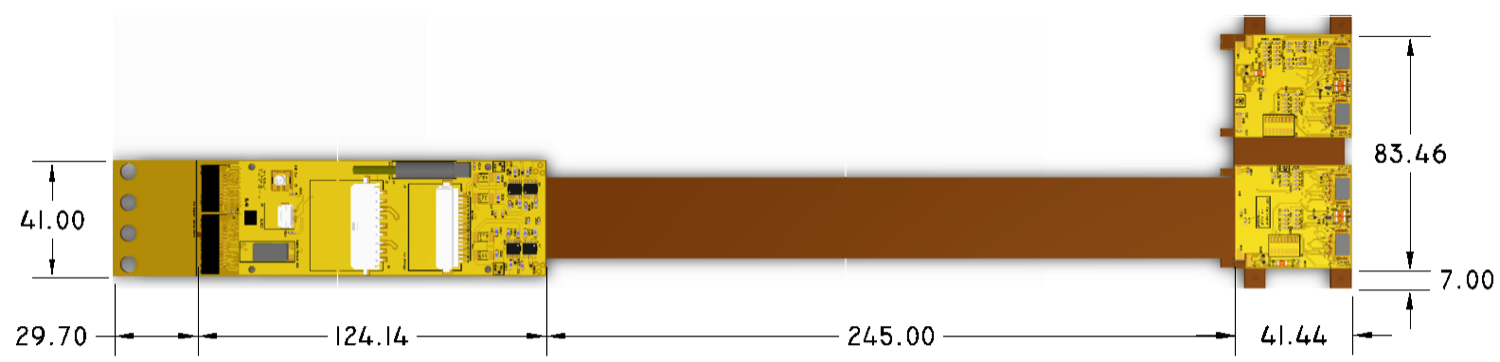
\includegraphics[width=1.0\columnwidth]{HFCB.png}
\caption{Hybrid Flex Circuit Board (HFCB).Level one connect board (left side) is connected to the hybrid area (right side)}
\label{fig:HFCB}
\end{figure}

Both sides of a module are instrumented with a readout system by a single rigid-flex Hybrid Flex Circuit Board (HFCB) located on the upstream end of the module (see Fig.~\ref{fig:HFCB}). HFCB provides bias to the silicon sensors, power and control lines to four FSSR2 ASICs located at the edge of the hybrid, two on the top and two on the bottom side. The ASICs are fixed to pads on their substrates with conductive epoxy. These pads are the reference for the analog return for the chips. The hybrid area of HFCB (42 x 82 mm) consists of two rigid boards (top and bottom hybrids) connected by a 10~mm-long wing flex High Density Interconnect (HDI) cable wrapped around the backing structure (Fig.~\ref{fig:hfcb-wrap}). Both hybrids connect to the module electrically using micro-bonding technology for the signals and bias return, and solder connection for the detector bias and module support ground. The sensors, the pitch adapters, and the HFCB are glued to both sides of the backing structure. 

\begin{figure}[hbt] 
\centering 
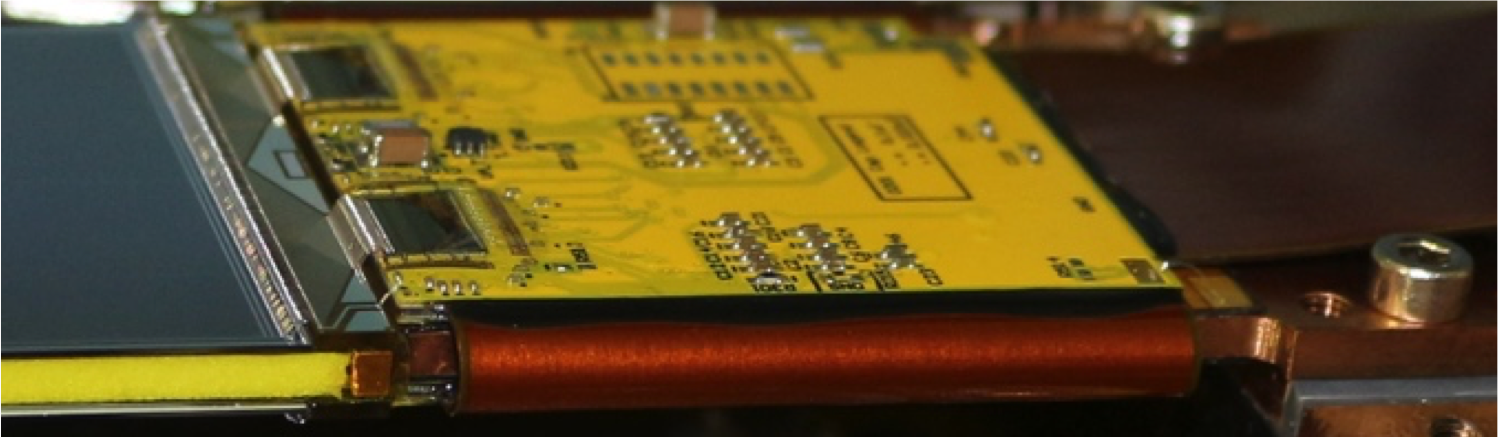
\includegraphics[width=1.0\columnwidth,keepaspectratio]{hfcb-wrap.png}
\caption{HFCB wrap}
\label{fig:hfcb-wrap}
\end{figure}

Module services are provided via the level one connect (L1C) board (125 x 41 mm) coupled to the hybrid area via the upstream flex HDI cable (245 mm). The upstream flex HDI cable is routed through 10~mm radial slots in the cold plate. The L1C board hosts two high density Nanonics connectors for data and control lines, Molex Micro-Fit 9-pin connector for high voltage ($\sim$85~V) bias to the sensors, AMP Mini CT 17 pin connector for low voltage (2.5~V) power to the ASICs, hybrid temperature connector, external pulser connector, and four voltage regulators. L1C board is mounted to the support tube on its own support structure designed to keep each L1C board positioned in line with its module.

The HFCB layer stack up consist of six layers of flexible polyimide sandwiched between two triple layers of rigid FR4 (Flame Retardant glass-reinforced epoxy laminate material). The stack up varies from section to section, the flexible sections (wing and upstream flex) only contain the polyimide where as the rigid areas contain all 12 layers. This variation in stack up provides ability to instrument both top and bottom sides of a module and pass though the cold plate to the L1C board mounted on the support structure. The two outer layers of the flex stack are the top and bottom shields, they are solid copper pours used to improve signal integrity by providing shielding and references for the differential signals. The top and bottom layers are made from 1 oz copper, while all the inner layers are made from 0.5 oz copper. The thickness of the rigid boards is 1.42 mm, flex cable is 0.5 mm thick.

Separate planes are provided for analog and digital power on each side of the hybrid. To reduce noise on these planes, all chip voltage lines are decoupled from the LV return with capacitors near the chips. High voltage filter circuits and the bridging of high and low voltage return lines are located close to the ASICs. Decoupling capacitors for power transmission are placed at transitions between flex and rigid materials. All data, clock, status and register traces are routed with no crossing of the splits in the reference planes. All clock traces are separated from other differential signals by guard traces which are stitched to the ground planes with vias. The trace width of the guard is 10 mils. No clocks are routed under the chips. All power lines are  decoupled from the ground using 2.2 or 4.7$\mu$F capacitors close to a transition in the PCB material (flex to rigid). Sensor bias lines are separated from the data lines by the guard traces. Clocks are terminated at the end of the pair line with two 50 Ohm resistors in series between the LVDS pair, with a 0.1 $\mu$F termination capacitor at the node between the resistors and the ground. There are temperature sensors located between the two FSSR2 chips on each side of the HFCB for monitoring purposes. In the hybrid areas, the bottom layer is used to transfer heat from the chips to a copper insert built into the module support core.

\begin{figure}[hbt] 
\centering 
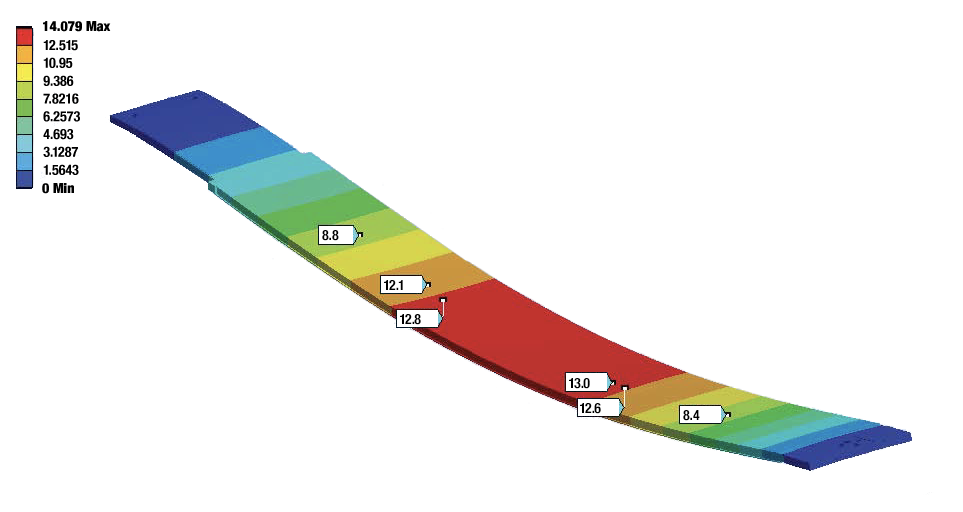
\includegraphics[width=1.0\columnwidth]{module-deflection.png}
\caption{Deflection of an individual module due to gravity.}
\label{fig:module-deflection}
\end{figure}

Thermal and structural FEA on SVT detector elements was performed using ANSYS. Deflection in the detector was analyzed for an individual module and for a region as a whole. The deflection was calculated based on gravitational load on the module. On the upstream end the module was assumed to be fixed since it is fastened to the upstream support ring of the detector. On the downstream end a simply supported condition was assumed since it is supported by the downstream ring. The maximum deflection of a module due to gravity is 14~$\mu$m (Figure~\ref{fig:module-deflection}). The deflection of the downstream ring is less than 7~$\mu$m. The vertical modules in the barrel minimize the deflection in the downstream ring making it a fairly rigid structure. The deflection of the entire SVT is 230~$\mu$m. 

For the thermal analysis, the module was modeled with the copper support and the heat sink insert. The heat output from each module is about 2.5 W. Cooling the cold plate with coolant flowing around the fins of the heat sink inserts inside the cold plate at -20$^\circ$C, at a rate of 2 liters per minute, results in a temperature differential of the coolant between the inlet and outlet of the cold plate to be less than 1$^\circ$C. The temperature distribution on the module is shown in Figure~\ref{fig:module-temp}. The maximum temperature of the sensors at the readout end is -10$^\circ$C. The variation in temperature from the upstream end of the Hybrid sensor to the downstream end of the Far sensor is about 1$^\circ$C.

\begin{figure}[hbt] 
\centering 
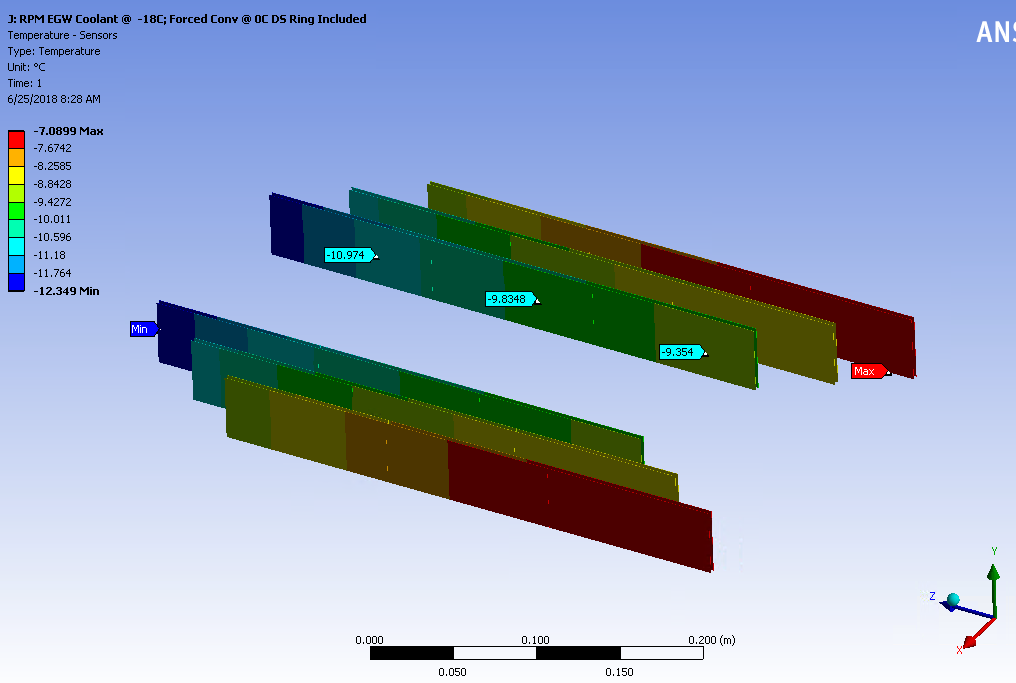
\includegraphics[width=1.0\columnwidth,keepaspectratio]{module-temp.png}
\caption{Temperature distribution along the SVT module.}
\label{fig:module-temp}
\end{figure}
%\begin{wrapfigure}{l}{0.5\columnwidth}
%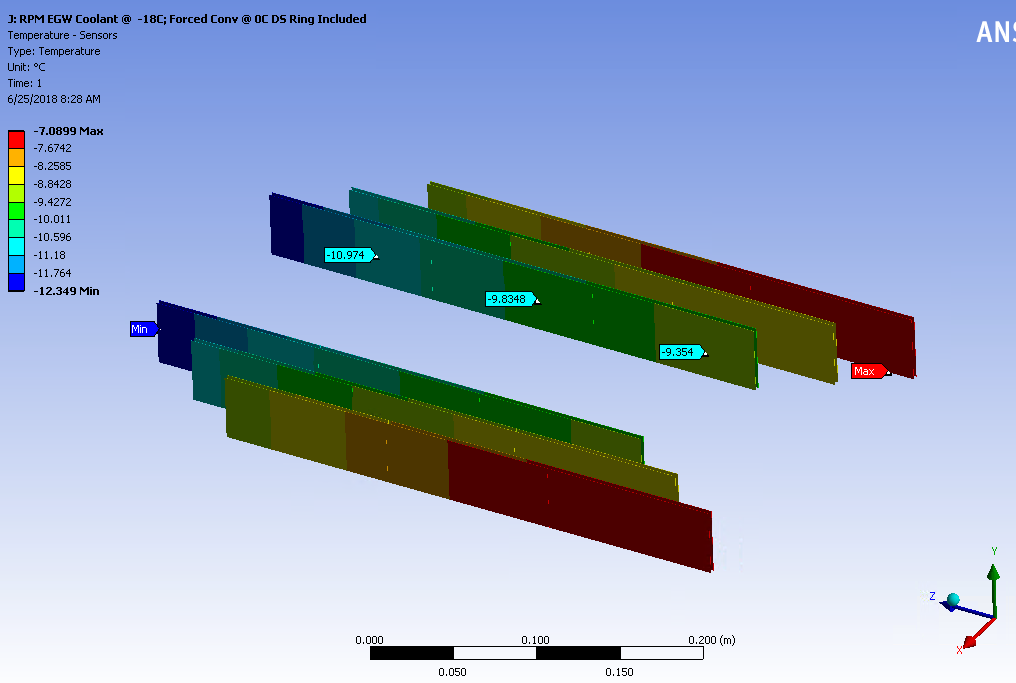
\includegraphics[width=1.0\columnwidth]{module-temp.png}
%\caption{Temperature distribution along the SVT module.}
%\label{fig:module-temp}
%\end{wrapfigure}

\subsection{Module Assembly and QA}

SVT modules are assembled at the Fermilab Silicon Detector Facility and tested at the Jefferson Lab. Prior to installation on a module, all components are inspected and tested as part of the quality assurance procedure.  
The layout of six bus cables on a panel has a minimum of 5.05 mm between adjacent cables on the panel to allow for the 1/8-inch diameter routing bit (Figure~\ref{fig:bus-cable-routing}).

To assemble the backing structure, a mold and an epoxy that cures at room temperature are used. Backing structures are cured on precision jig to satisfy required tolerances. The module has two pairs of mounting and fiducial holes in the copper heat sink and one in the PEEK insert. After module is fabricated, position of these fiducial holes is measured with respect to the fiducial marks etched on the sensor. Sensors are aligned with respect to insert fiducials within few micrometers. The holes for the mounting pin have a tight diameter tolerance and are used for module alignment. The slot in the PEEK insert has a tolerance of 5~$\mu$m. To accurately control the width of the backing structure, post-machining of the width at the downstream end and near the pitch adapter is done. After post-machining of the precision edge, any foam exposed due to that process is encapsulated with 3M DP190 epoxy. Edges of the backing structure are covered with Kapton tape to insulate the carbon fiber from the back side of the sensors. After installation of the HFCBs and pitch adapters, the module is placed in a box designed to allow storage of partially and fully fabricated modules.

%\begin{figure}[hbt] 
%\centering 
%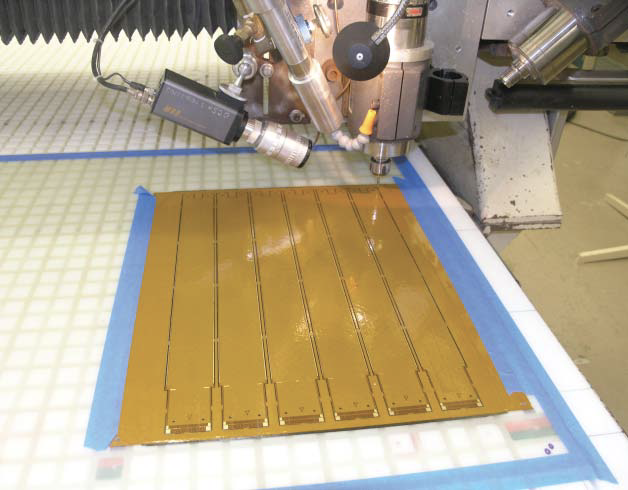
\includegraphics[width=1.0\columnwidth,keepaspectratio]{bus-cable-routing.png}
%\caption{Cutting of the bus cable.}
%\label{fig:bus-cable-routing}
%\end{figure}
\begin{figure}[hbt] 
\centering 
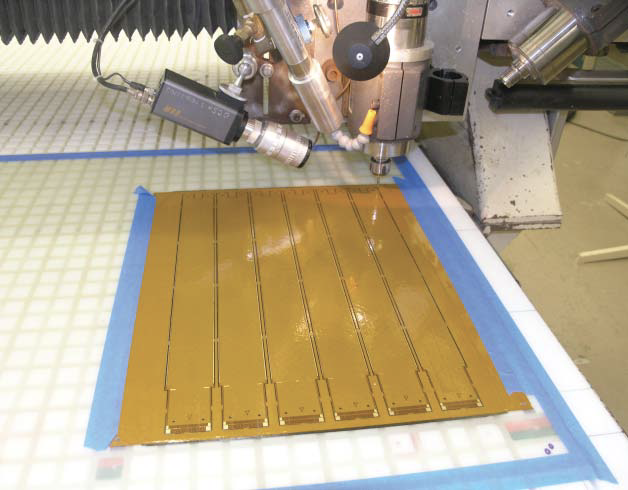
\includegraphics[width=1.0\columnwidth,keepaspectratio]{bus-cable-routing.png}
\caption{Cutting of the bus cable.}
\label{fig:bus-cable-routing}
\end{figure}

Module performance tests were done at various stages during module production at Fermilab and during assembly of the SVT at Jefferson Lab. 

The position resolution of the detector can be compromised if the alignment is not known. Due to tight material budget restrictions there is no room for individual module adjustment system. Strict positional tolerances are imposed so that minimal corrections need to be made to measurements. Therefore, both the position of the sensors with respect to each other and with respect to alignment points are measured and controlled during module production. A mechanical survey is  carried out before electrical testing to check that the module fits within a well-defined envelope and ensure no interference with adjacent modules on the support structure.

After assembly the modules are mounted inside carrier boxes, transported to Jefferson Lab and re-tested. The module can be powered, cooled (using passive heat sink), and operated in the carrier box. The carrier box allows access to both sides of the module to facilitate inspection and debugging.

\subsection{Detector integration and commissioning}

%\begin{figure}[hbt]
%\centering 
%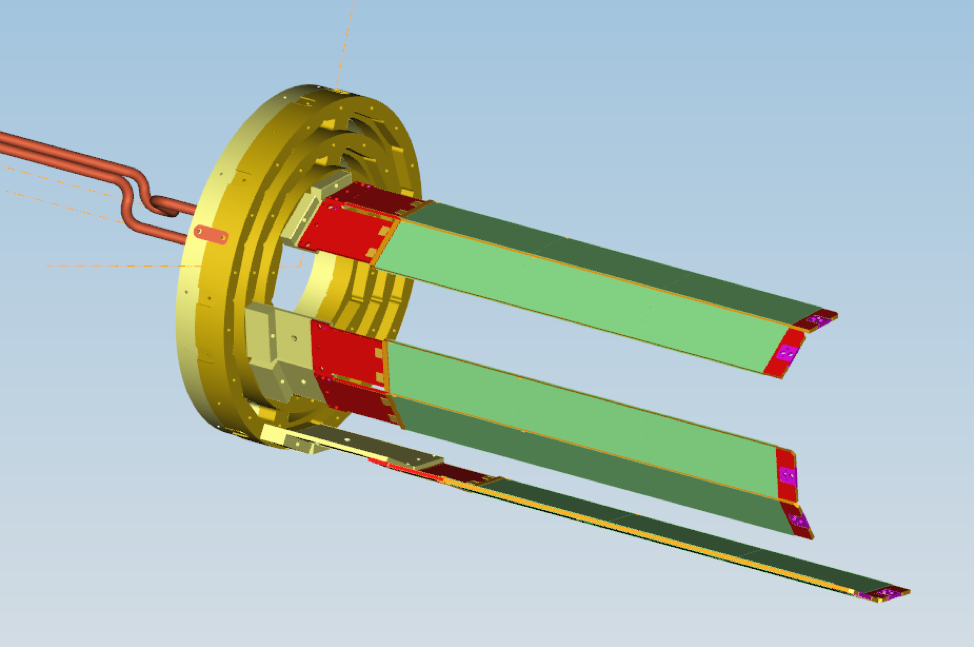
\includegraphics[width=1.0\columnwidth,keepaspectratio]{modulesupport.png}
%\caption{SVT barrel assembly.}
%\label{fig:modulesupport}
%\end{figure}
Barrel integration took place at the Jefferson Lab. Regions are assembled in sequence. The assembly was done in a vertical position on a granite table. Region 1 (innermost region) is assembled first, followed by Regions 2 and 3. Modules are mounted on the dowels inserted in the rings by holding the module by the two handling rods which are screwed into the inserts (Fig.~\ref{fig:svt-assembly}). 

\begin{figure}[hbt] 
\centering 
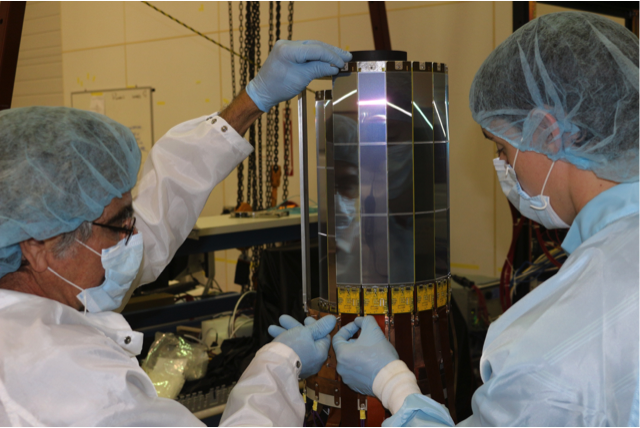
\includegraphics[width=1.0\columnwidth,keepaspectratio]{svt-assembly.png}
\caption{SVT assembly}
\label{fig:svt-assembly}
\end{figure}

The upstream support ring is fastened to the cold plate by a single screw for each of the copper module supports. This ensures good thermal contact between the inserts on the cold plate and the module supports of the upstream support ring. A layer of thermal grease is applied between the mating surfaces. The cold plate and upstream ring are then mounted to a mounting tube. The larger flange on the mounting tube rests on the granite table. 

\begin{figure}[hbt] 
\centering 
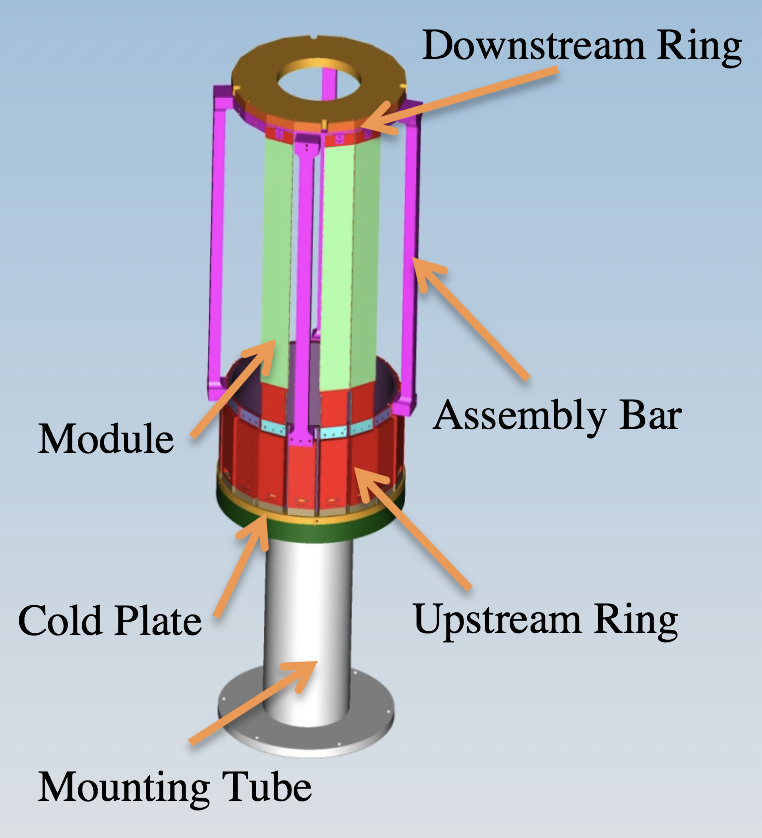
\includegraphics[width=1.0\columnwidth,keepaspectratio]{barrel-integration.png}
\caption{Region assembly}
\label{fig:barrel-integration}
\end{figure}

The downstream ring is supported by four aluminum region assembly bars (Fig.~\ref{fig:barrel-integration}) fastened to it to provide stiffness to the ring during assembly. These bars have accurately positioned holes and precision mounting surfaces to position the downstream ring. As the modules are mounted around the polygonal rings the assembly bars are replaced by the modules one at a time. The mounting surfaces of the upstream and downstream rings are machined simultaneously to reduce twist in the module which could result from the two surfaces not being co-planar. The holes for locating pins and tapped holes for fasteners on the upstream and downstream ring are also added at this stage. Once the downstream ring is in position, the CMM is used to establish a coordinate system for the detector and a central axis for the detector based on fiducials machined onto the flange of the mounting tube and the tooling plate on the downstream ring. The downstream ring has holes into it for accommodating dowels and screws used for locating and mounting the module on the downstream end. The module has a slot machined into it which accommodates the locating dowel. This constrains the module in the tangential direction without constraining it in the axial direction as seen in Fig.~\ref{fig:downstreamring}. 

\begin{figure}[hbt] 
\centering 
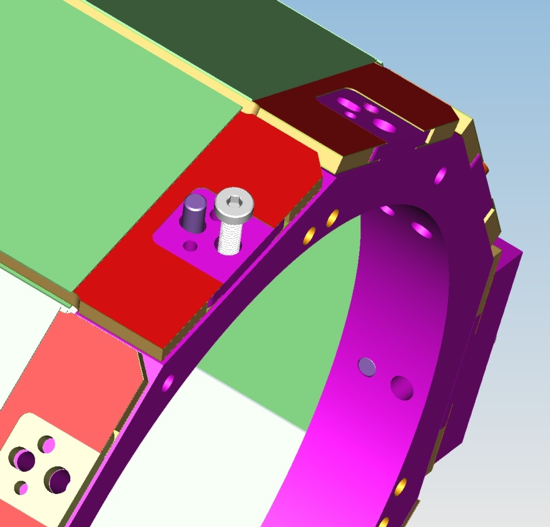
\includegraphics[width=1.0\columnwidth,keepaspectratio]{downstreamring.png}
\caption{Downstream support of the module.}
\label{fig:downstreamring}
\end{figure}

The other holes are used for surveying the module location and for handling the module during assembly. There are three fiducial points on each module, two on the upstream copper insert, and one on the downstream PEEK insert. Upon completion of each region, the locations of fiducials on the downstream and upstream rings are measured with respect to the coordinate axes with precision of $\sim$20~$\mu$m using a FaroArm Quantum CMM. The shifts of survey positions from ideal geometry were taken into account by the alignment software. Upon completion of the assembly of all modules the detector is moved to a horizontal position and the relative positions between the downstream rings of all three regions are measured and recorded.
%(see Fig.~\ref{fig:survey}).
%\begin{figure}[hbt] 
%\centering 
%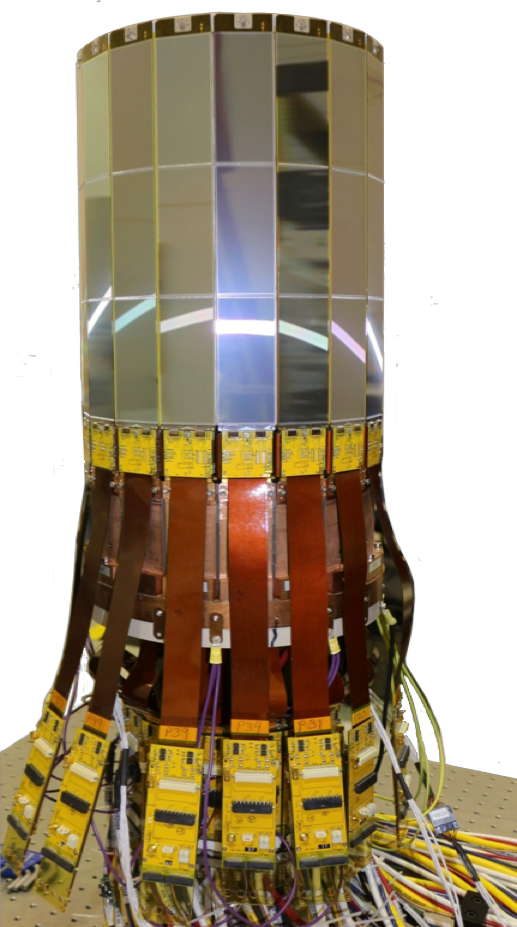
\includegraphics[width=0.3\columnwidth,keepaspectratio]{barrel-assembled.png}
%\caption{Assembled barrel}
%\label{fig:barrel-assembled}
%\end{figure}

After placement of each module on the support, all the modules on the support are re-tested to find and resolve problems with cables routed on the outside of the cylinder. Once assembly is completed, a light-tight Faraday cage encloses the SVT, dry air is flushed through it and the modules are cooled. 

%\begin{wrapfigure}{l}{0.5\columnwidth}
%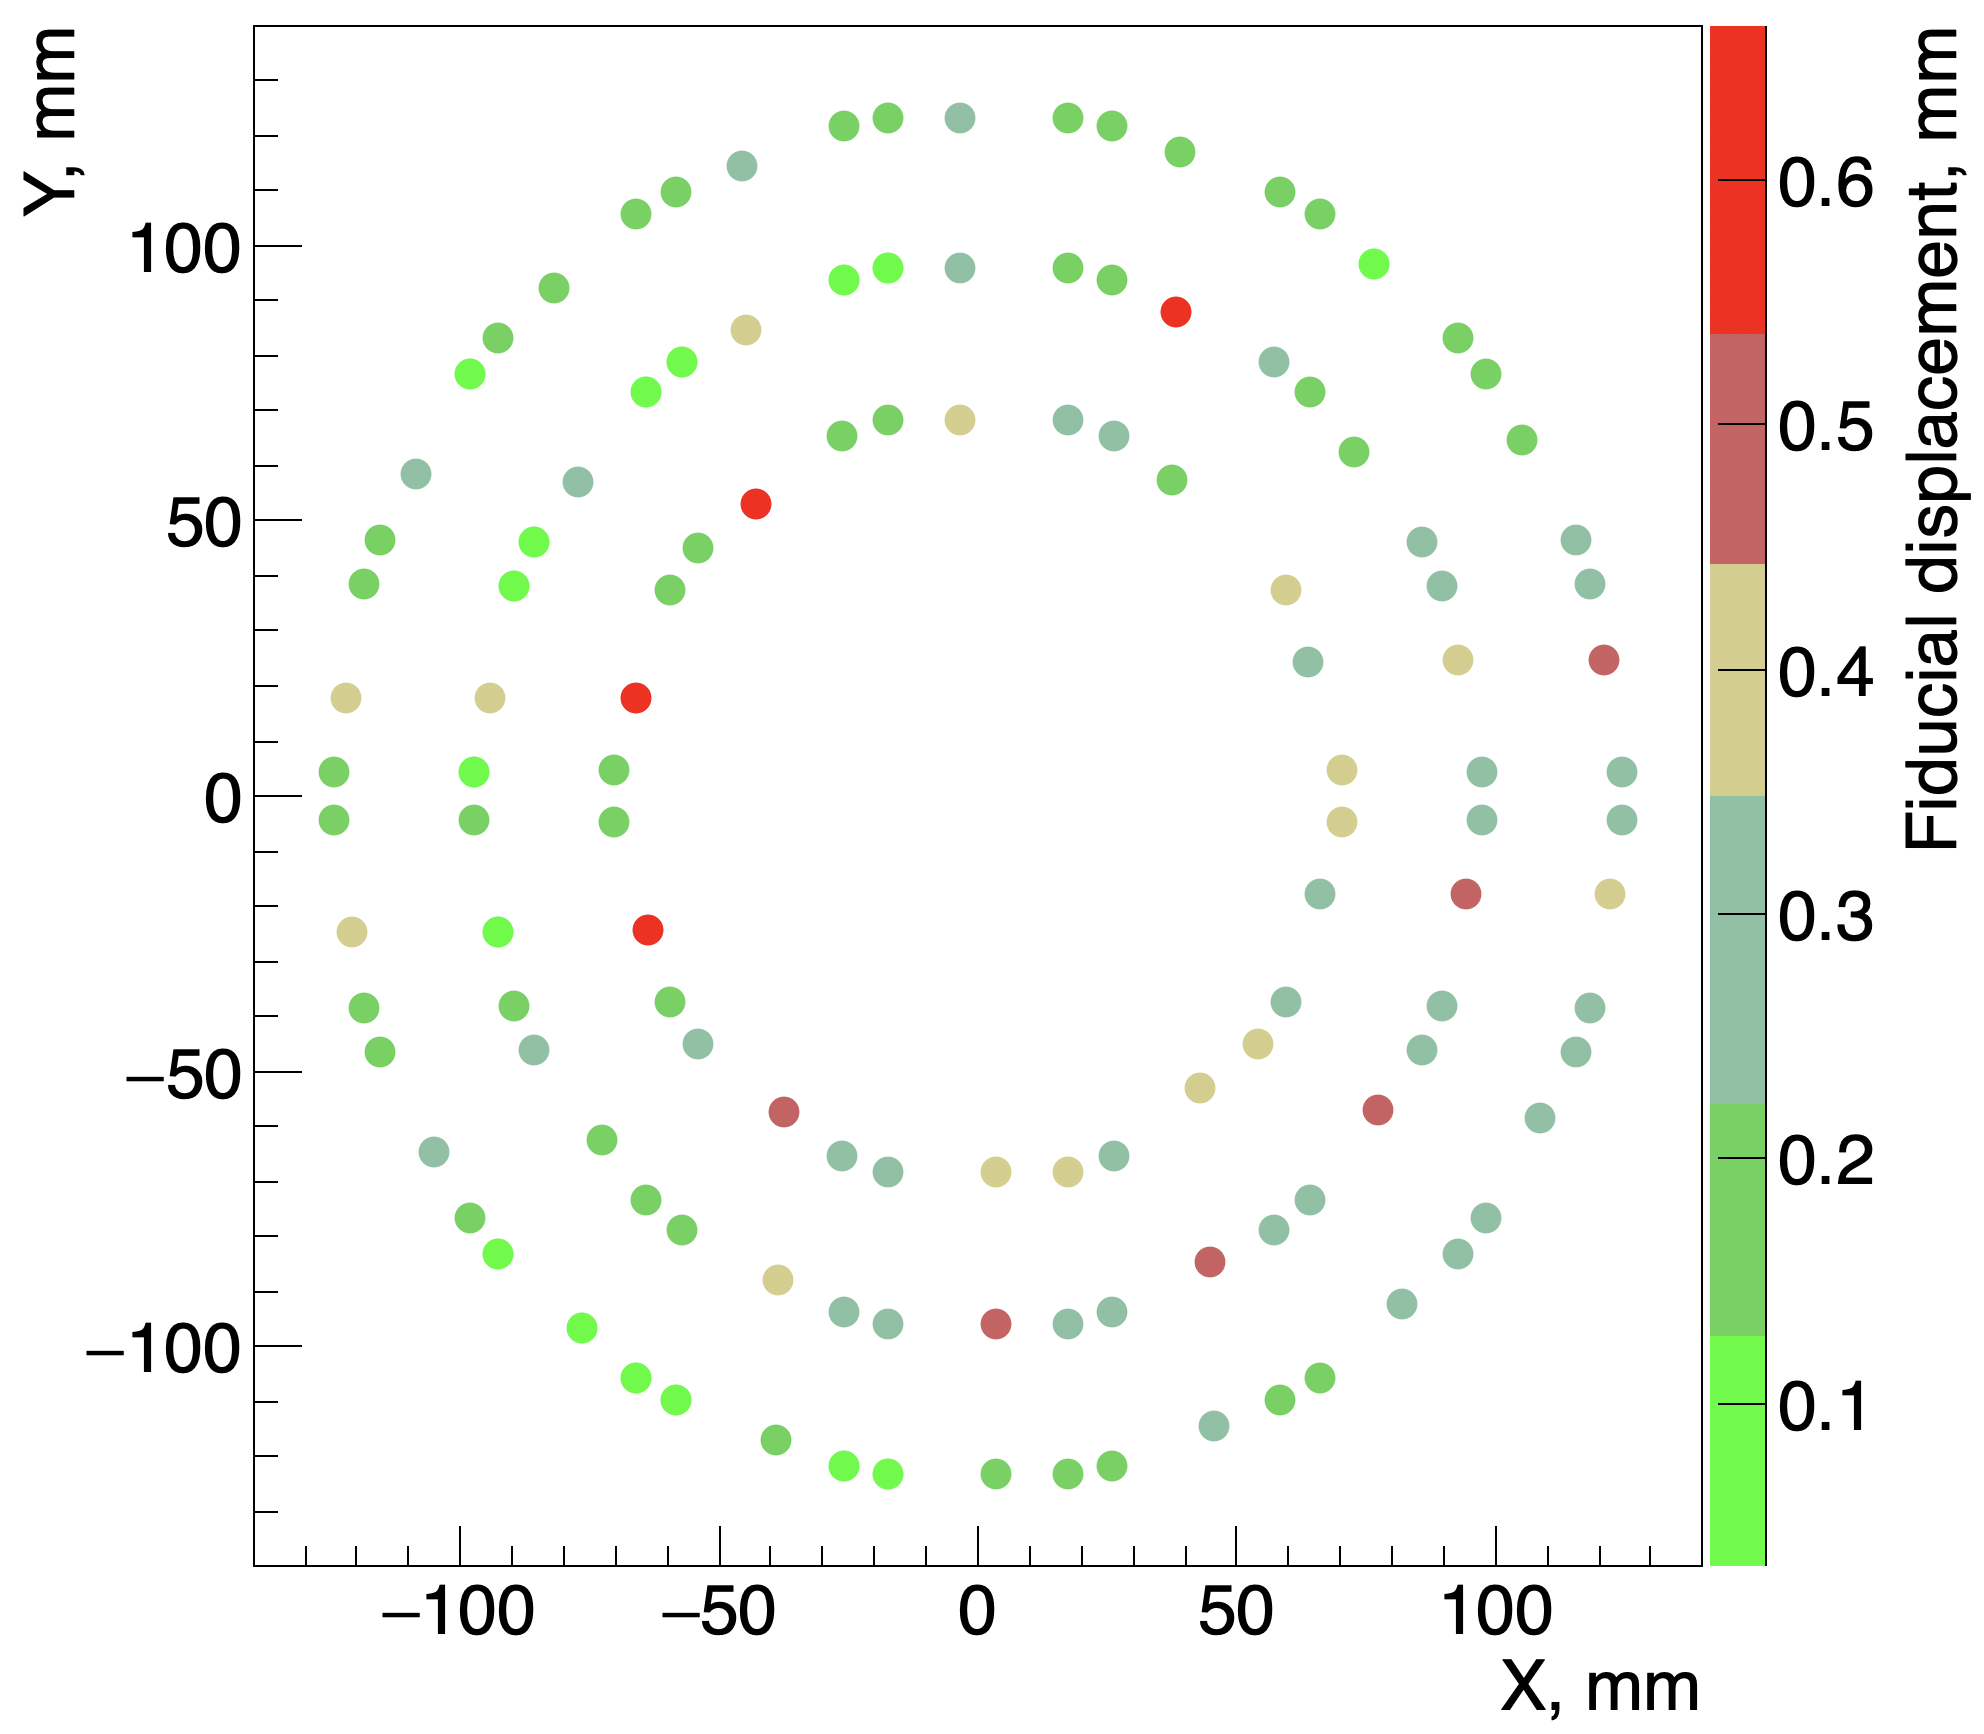
\includegraphics[width=1.0\columnwidth]{survey.png}
%\caption{Survey}
%\label{fig:survey}
%\end{wrapfigure}
%
%(Fig.~\ref{fig:barrel-assembled}) 

\begin{figure}[hbt] 
\centering 
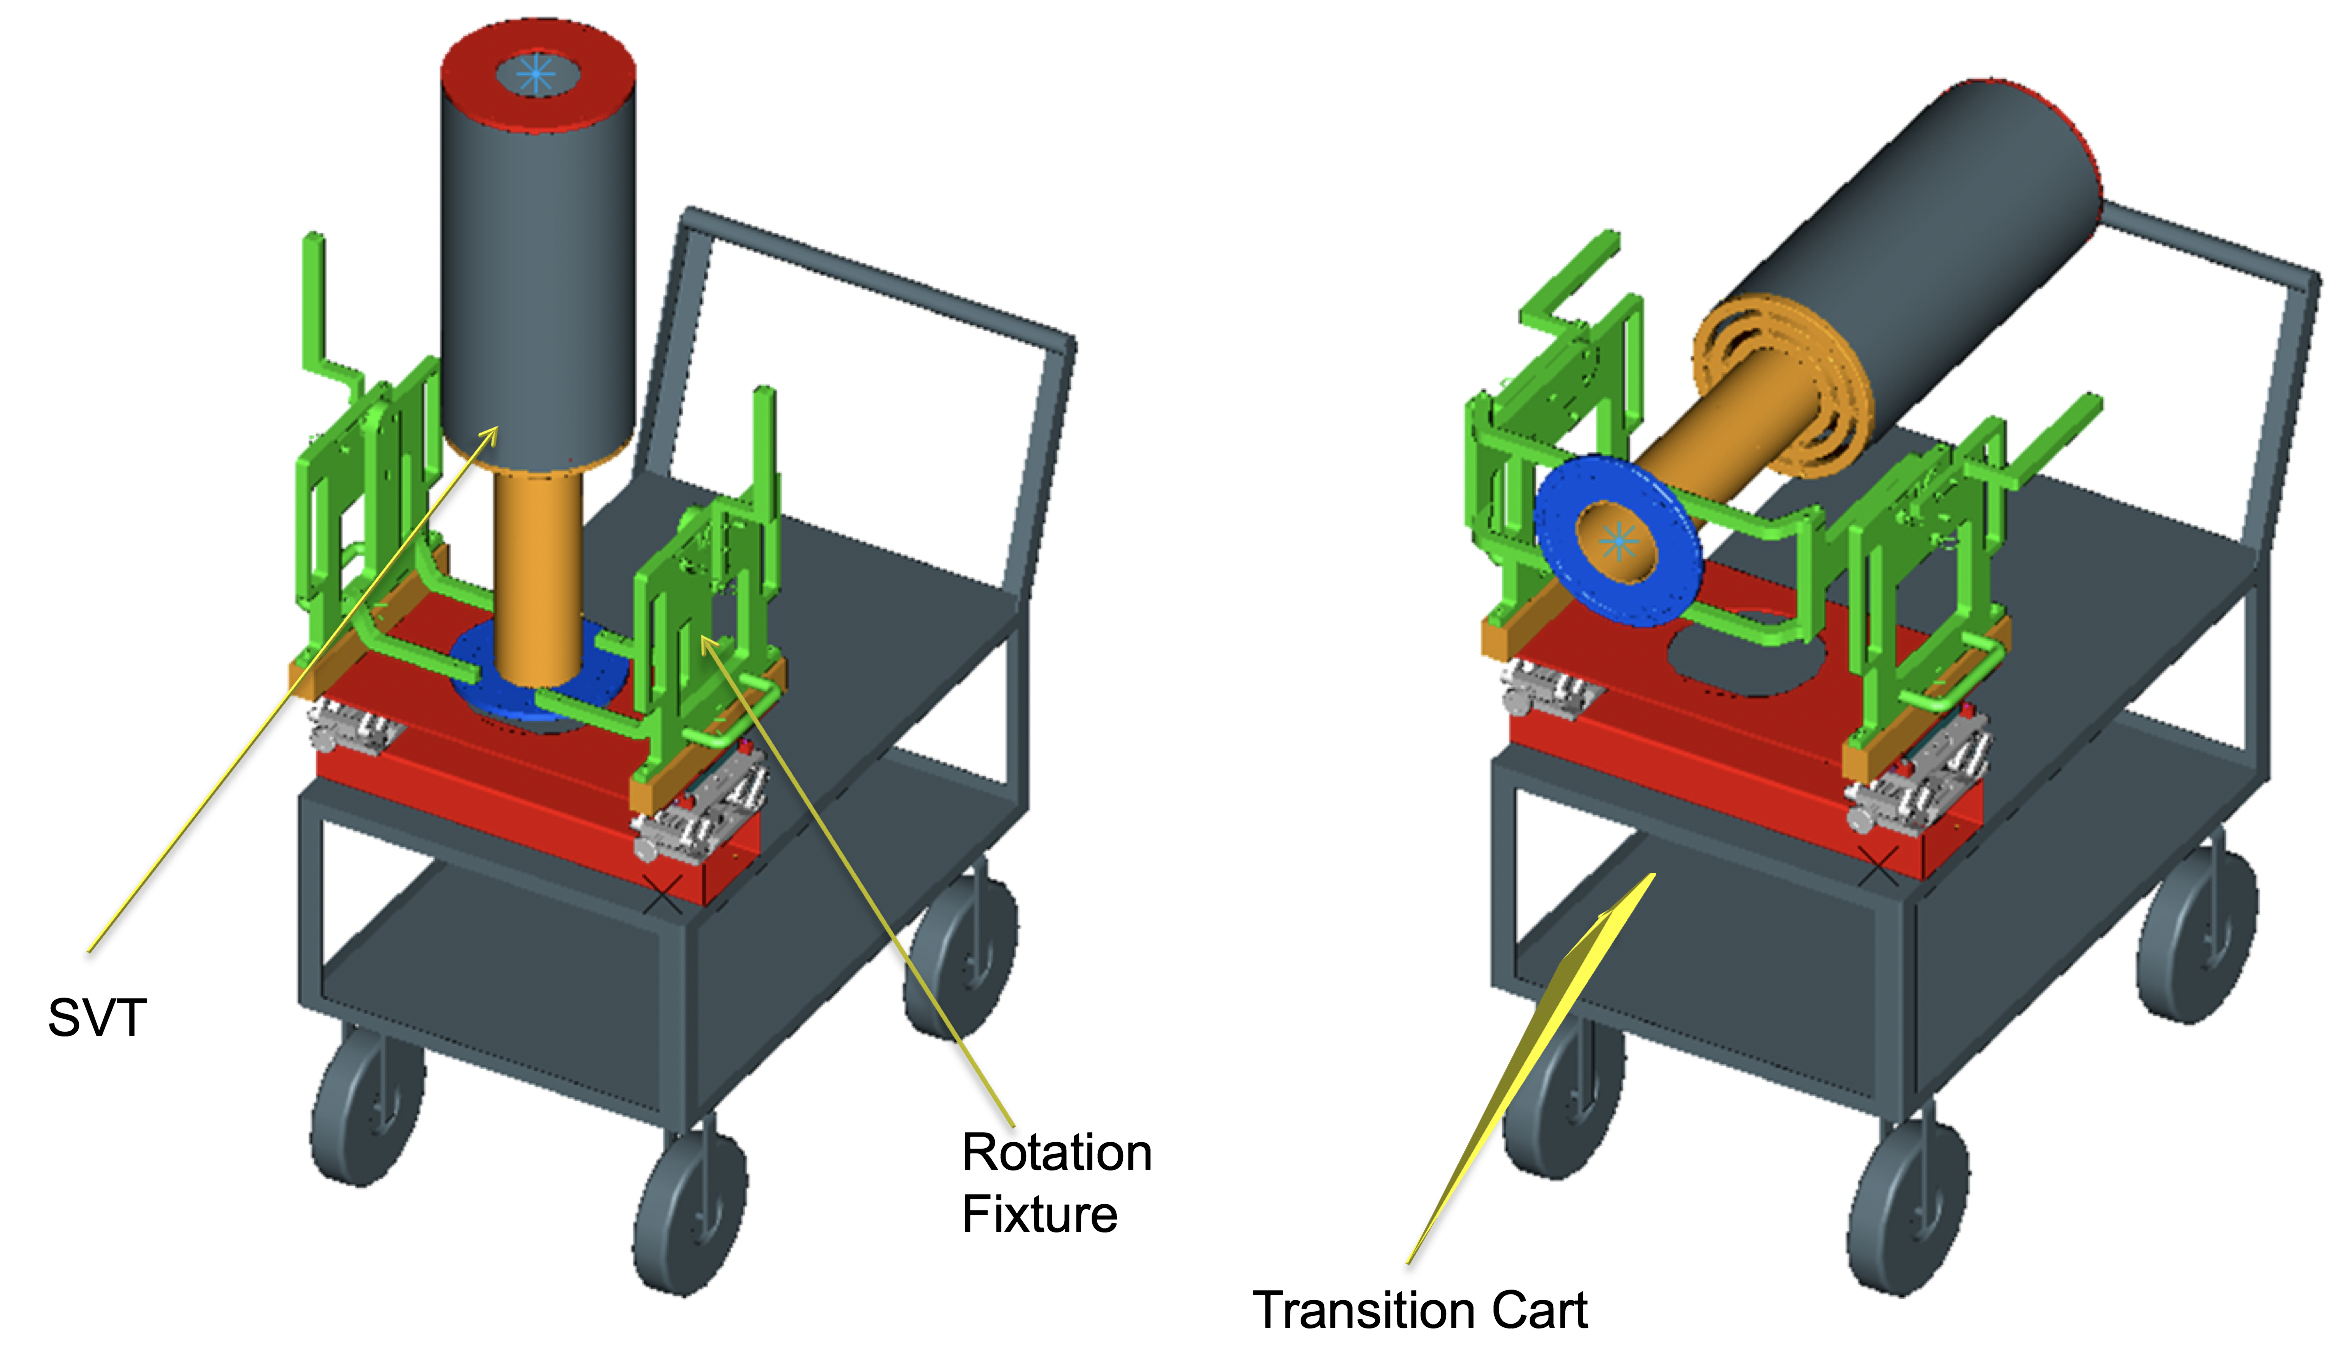
\includegraphics[width=1.0\columnwidth,keepaspectratio]{rotation-fixture.png}
\caption{Barrel rotation with transition fixture.}
\label{fig:rotation-fixture}
\end{figure}

After assembling each region the functionality of integrated modules was checked. When barrel assembly was complete, it was rotated to a horizontal position using a special transition fixture (Fig.~\ref{fig:rotation-fixture}). 

SVT support tube was mounted on the integration cart (Fig.~\ref{fig:integration-cart}) using a crane and mounting fixture placed on the parallel rails. The adjustment links on the cart allow for the SVT to be aligned with the support tube. The survey of the fiducials on the support structure was performed and alignment of the barrel was done by shimming the support tube and adjusting the mounting fixture links. 

\begin{figure}[hbt] 
\centering 
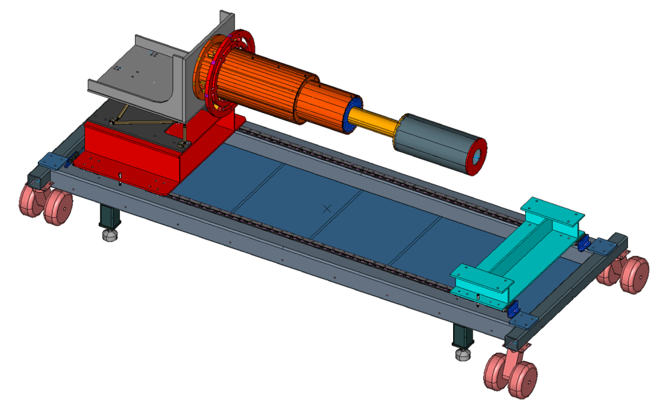
\includegraphics[width=1.0\columnwidth,keepaspectratio]{integration-cart.png}
\caption{Integration cart.}
\label{fig:integration-cart}
\end{figure}

The mounting fixture with attached barrel was moved to one side of the integration card and locked into place. At this time, cables and cooling lines are connected to the SVT (Fig.~\ref{fig:svt-assembled}). Cable bundles were secured to the support tube using the nylon eyebolts on the tube and connected to the crates. 

\begin{figure}[hbt] 
\centering 
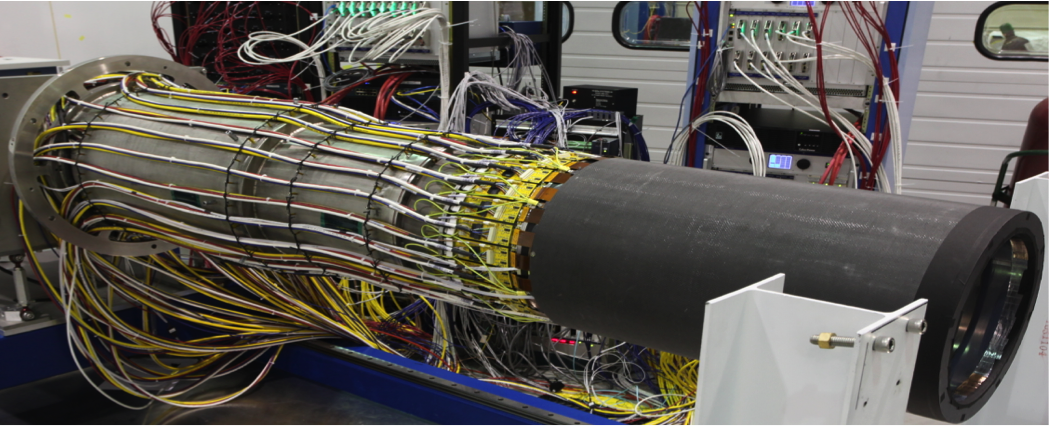
\includegraphics[width=1.0\columnwidth,keepaspectratio]{svt-assembled.png}
\caption{SVT barrel after integration.}
\label{fig:svt-assembled}
\end{figure}

The detector was tested and commissioned with cosmic rays. Integration cart was enclosed in the protective cover, the wheels are placed in the suspension pods and the cart was transported to the experimental hall on the track. In the hall the SVT was craned off the integration cart and mounted on the service cart. The cart hosts all detector services and is movable along the beam axis for easy maintenance.

After installation in Hall B, the SVT was tested with the services that are used to operate the SVT during the data-taking. A series of runs were performed with and without the beam and with and without the magnetic field, four configurations in all. For each of these configurations, the tests for the module performance were repeated. Tests at later stages aimed at finding problems with data acquisition and services, such as the power supplies and cables, and ensuring that no common mode noise was added to the system due to improper grounding and shielding. 

